\documentclass{article}

% Packages
\usepackage{amsmath}
\usepackage{amsfonts}
\usepackage{amssymb}
\usepackage{geometry}
\usepackage{tikz}
\usepackage{float}
\usepackage{enumitem}
\usepackage{mathtools}
\usepackage{subcaption}
\usepackage[colorlinks=true]{hyperref}
\usepackage{forest}
\usepackage[]{multicol}


\forestset{
dg edges/.style={for tree={parent anchor=south, child anchor=north,align=center,base=bottom,where n children=0{tier=word,edge=dotted,calign with current edge}{}}},
}
% \usetikzlibrary{automata, arrows.meta, positioning,shapes}

\numberwithin{equation}{subsection}
\renewcommand{\thesubsection}{\thesection.\arabic{subsection}}
% \renewcommand{\thesubsubsection}{\Alph{subsubsection}}

\newcommand{\setsubsubsectionnumber}[1]{\setcounter{subsubsection}{#1}\addtocounter{subsubsection}{-1}}

\DeclareMathOperator{\putx}{put}

\makeatletter
\newcommand{\leqnomode}{\tagsleft@true}
\newcommand{\reqnomode}{\tagsleft@false}
\makeatother

\newcommand{\abs}[1]{\vert #1\vert}
\newcommand{\tab}[1][30pt]{\hspace*{#1}}
\newcommand{\bracket}[1]{\biggl[#1\biggr]}

\title{Theory of Machines and Languages Homework 4}
\author{Ali Abbasi}
\begin{document}
\maketitle
\tableofcontents
\pagebreak

\section{Turing Machines and Turing Recognizable Languages}
\subsection{}
We cross the first \(a\), go to the first \(b\) and cross it, go back to first \(a\) and repeat, until all \(a\)s are crossed.
Then check that rest of the string (that is not crossed yet) contains only \(b\)s and if so, accept the string.
\begin{figure}[H]
\centering
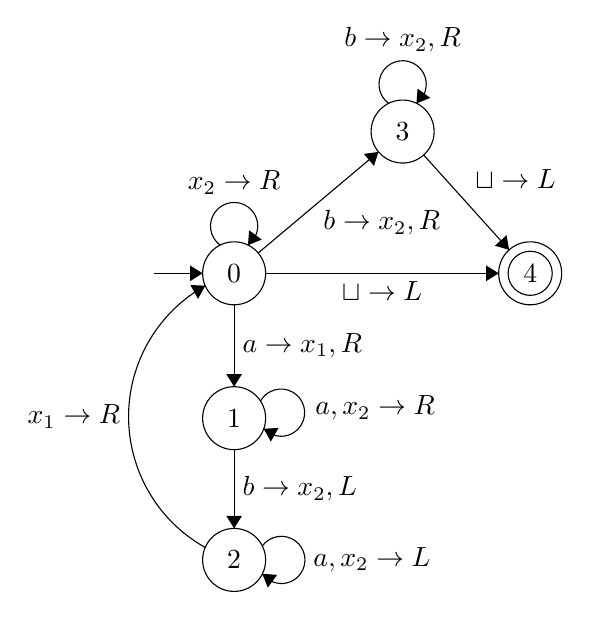
\begin{tikzpicture}[scale=0.2]
    \tikzstyle{every node}+=[inner sep=0pt]
    \draw [black] (12.9,-15.9) circle (2);
    \draw (12.9,-15.9) node {$0$};
    \draw [black] (12.9,-25.1) circle (2);
    \draw (12.9,-25.1) node {$1$};
    \draw [black] (12.9,-34.1) circle (2);
    \draw (12.9,-34.1) node {$2$};
    \draw [black] (31.7,-15.9) circle (2);
    \draw (31.7,-15.9) node {$4$};
    \draw [black] (31.7,-15.9) circle (1.4);
    \draw [black] (23.6,-6.9) circle (2);
    \draw (23.6,-6.9) node {$3$};
    \draw [black] (7.8,-15.9) -- (10.9,-15.9);
    \fill [black] (10.9,-15.9) -- (10.1,-15.4) -- (10.1,-16.4);
    \draw [black] (12.9,-17.9) -- (12.9,-23.1);
    \fill [black] (12.9,-23.1) -- (13.4,-22.3) -- (12.4,-22.3);
    \draw (13.4,-20.5) node [right] {$a\to x_1,R$};
    \draw [black] (12.9,-27.1) -- (12.9,-32.1);
    \fill [black] (12.9,-32.1) -- (13.4,-31.3) -- (12.4,-31.3);
    \draw (13.4,-29.6) node [right] {$b\to x_2,L$};
    \draw [black] (14.571,-24.016) arc (150.71173:-137.28827:1.5);
    \draw (18.03,-24.46) node [right] {$a,x_2\to R$};
    \fill [black] (14.78,-25.77) -- (15.23,-26.59) -- (15.72,-25.72);
    \draw [black] (14.686,-33.218) arc (144:-144:1.5);
    \draw (17.9,-34.1) node [right] {$a,x_2\to L$};
    \fill [black] (14.69,-34.98) -- (15.04,-35.86) -- (15.63,-35.05);
    \draw [black] (11.066,-33.311) arc (-119.29474:-240.70526:9.53);
    \fill [black] (11.07,-16.69) -- (10.12,-16.64) -- (10.61,-17.52);
    \draw (5.7,-25) node [left] {$x_1\to R$};
    \draw [black] (12.018,-14.114) arc (234:-54:1.5);
    \draw (12.9,-10.9) node [above] {$x_2\to R$};
    \fill [black] (13.78,-14.11) -- (14.66,-13.76) -- (13.85,-13.17);
    \draw [black] (14.9,-15.9) -- (29.7,-15.9);
    \fill [black] (29.7,-15.9) -- (28.9,-15.4) -- (28.9,-16.4);
    \draw (22.3,-16.4) node [below] {$\sqcup\to L$};
    \draw [black] (14.43,-14.61) -- (22.07,-8.19);
    \fill [black] (22.07,-8.19) -- (21.14,-8.32) -- (21.78,-9.08);
    \draw (22.28,-11.89) node [below] {$b\to x_2,R$};
    \draw [black] (22.718,-5.114) arc (234:-54:1.5);
    \draw (23.6,-1.9) node [above] {$b\to x_2,R$};
    \fill [black] (24.48,-5.11) -- (25.36,-4.76) -- (24.55,-4.17);
    \draw [black] (24.94,-8.39) -- (30.36,-14.41);
    \fill [black] (30.36,-14.41) -- (30.2,-13.48) -- (29.46,-14.15);
    \draw (28.19,-9.94) node [right] {$\sqcup\to L$};
    \end{tikzpicture}
\caption{Turing machine for the language \(L= \left\{a^mb^n\mid 0\le m\le n\right\}\).}
\end{figure}
Transitions of the shape \(a\to R\) which don't mention what character to write, just leave the character intact (or write the same character).

\subsubsection{}
\begin{figure}[H]
\centering
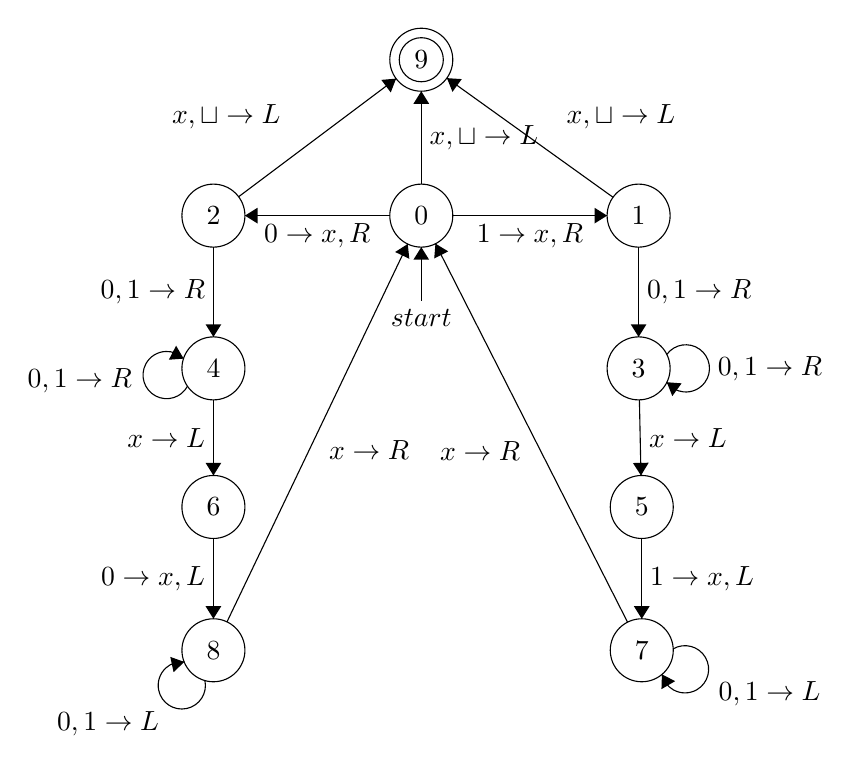
\begin{tikzpicture}[scale=0.2]
    \tikzstyle{every node}+=[inner sep=0pt]
    \draw [black] (25,-12.1) circle (2);
    \draw (25,-12.1) node {$0$};
    \draw [black] (38.8,-12.1) circle (2);
    \draw (38.8,-12.1) node {$1$};
    \draw [black] (11.8,-12.1) circle (2);
    \draw (11.8,-12.1) node {$2$};
    \draw [black] (38.8,-21.8) circle (2);
    \draw (38.8,-21.8) node {$3$};
    \draw [black] (11.8,-21.8) circle (2);
    \draw (11.8,-21.8) node {$4$};
    \draw [black] (39,-30.6) circle (2);
    \draw (39,-30.6) node {$5$};
    \draw [black] (39,-39.7) circle (2);
    \draw (39,-39.7) node {$7$};
    \draw [black] (11.8,-30.6) circle (2);
    \draw (11.8,-30.6) node {$6$};
    \draw [black] (11.8,-39.7) circle (2);
    \draw (11.8,-39.7) node {$8$};
    \draw [black] (25,-2.2) circle (2);
    \draw (25,-2.2) node {$9$};
    \draw [black] (25,-2.2) circle (1.4);
    \draw [black] (25,-17.5) -- (25,-14.1);
    \draw (25,-18) node [below] {$start$};
    \fill [black] (25,-14.1) -- (24.5,-14.9) -- (25.5,-14.9);
    \draw [black] (27,-12.1) -- (36.8,-12.1);
    \fill [black] (36.8,-12.1) -- (36,-11.6) -- (36,-12.6);
    \draw (31.9,-12.6) node [below] {$1\to x,R$};
    \draw [black] (23,-12.1) -- (13.8,-12.1);
    \fill [black] (13.8,-12.1) -- (14.6,-12.6) -- (14.6,-11.6);
    \draw (18.4,-12.6) node [below] {$0\to x,R$};
    \draw [black] (38.8,-14.1) -- (38.8,-19.8);
    \fill [black] (38.8,-19.8) -- (39.3,-19) -- (38.3,-19);
    \draw (39.3,-16.95) node [right] {$0,1\to R$};
    \draw [black] (11.8,-14.1) -- (11.8,-19.8);
    \fill [black] (11.8,-19.8) -- (12.3,-19) -- (11.3,-19);
    \draw (11.3,-16.95) node [left] {$0,1\to R$};
    \draw [black] (40.586,-20.918) arc (144:-144:1.5);
    \draw (43.8,-21.8) node [right] {$0,1\to R$};
    \fill [black] (40.59,-22.68) -- (40.94,-23.56) -- (41.53,-22.75);
    \draw [black] (38.85,-23.8) -- (38.95,-28.6);
    \fill [black] (38.95,-28.6) -- (39.44,-27.79) -- (38.44,-27.81);
    \draw (39.43,-26.2) node [right] {$x\to L$};
    \draw [black] (39,-32.6) -- (39,-37.7);
    \fill [black] (39,-37.7) -- (39.5,-36.9) -- (38.5,-36.9);
    \draw (39.5,-35.15) node [right] {$1\to x,L$};
    \draw [black] (40.99,-39.612) arc (120.27317:-167.72683:1.5);
    \draw (43.85,-42.49) node [right] {$0,1\to L$};
    \fill [black] (40.28,-41.23) -- (40.25,-42.17) -- (41.12,-41.66);
    \draw [black] (38.1,-37.92) -- (25.9,-13.88);
    \fill [black] (25.9,-13.88) -- (25.82,-14.82) -- (26.71,-14.37);
    \draw (31.31,-27.02) node [left] {$x\to R$};
    \draw [black] (11.8,-23.8) -- (11.8,-28.6);
    \fill [black] (11.8,-28.6) -- (12.3,-27.8) -- (11.3,-27.8);
    \draw (11.3,-26.2) node [left] {$x\to L$};
    \draw [black] (10.156,-22.925) arc (-27.8699:-315.8699:1.5);
    \draw (6.66,-22.61) node [left] {$0,1\to R$};
    \fill [black] (9.91,-21.18) -- (9.43,-20.36) -- (8.97,-21.25);
    \draw [black] (11.8,-32.6) -- (11.8,-37.7);
    \fill [black] (11.8,-37.7) -- (12.3,-36.9) -- (11.3,-36.9);
    \draw (11.3,-35.15) node [left] {$0\to x, L$};
    \draw [black] (11.26,-41.618) arc (12.01279:-275.98721:1.5);
    \draw (5.11,-43.53) node [below] {$0,1\to L$};
    \fill [black] (9.95,-40.44) -- (9.06,-40.12) -- (9.27,-41.09);
    \draw [black] (12.66,-37.9) -- (24.14,-13.9);
    \fill [black] (24.14,-13.9) -- (23.34,-14.41) -- (24.24,-14.84);
    \draw (19.11,-26.96) node [right] {$x\to R$};
    \draw [black] (25,-10.1) -- (25,-4.2);
    \fill [black] (25,-4.2) -- (24.5,-5) -- (25.5,-5);
    \draw (25.5,-7.15) node [right] {$x,\sqcup\to L$};
    \draw [black] (13.4,-10.9) -- (23.4,-3.4);
    \fill [black] (23.4,-3.4) -- (22.46,-3.48) -- (23.06,-4.28);
    \draw (12.62,-6.65) node [above] {$x,\sqcup\to L$};
    \draw [black] (37.17,-10.93) -- (26.63,-3.37);
    \fill [black] (26.63,-3.37) -- (26.98,-4.24) -- (27.57,-3.43);
    \draw (37.68,-6.65) node [above] {$x,\sqcup\to L$};
    \end{tikzpicture}
\caption{TM for the language \(L=\left\{w\in \left\{0, 1\right\}^*\mid w=w^R\right\}\)}
\end{figure}
Transitions from states 1 and 2 to the final state handle the case where the string has odd length.
\subsection{}
\subsubsection{}
We show that we can simulate a Turing Machine with a 2-stack pushdown automaton and vice versa.\\
\begin{itemize}
\item For simulating a Turing Machine with a 2-stack pushdown automaton, first we push the characters of the input string (\(s\)) as we read them to the first stack.
When we finish reading the input, we pop from the first stack and push to the second stack so that the characters are in the second stack in reverse order (we can push \$ to the stacks in the beginning so that we know when the stack is empty).
This is the initial configuration \(q_0s\).
Now we show how we go from one configuration to another configuration.\\
Suppose we are in the configuration \(C=xqy\); where \(q\) is the current state of the TM and its head points to the first character of \(y\) where \(y\) is in the second stack (in reverse order) and \(x\) is in the first stack.
\begin{itemize}[label=\(\circ\)]
\item \(\delta(q, a) = (q', b, L)\):
In this case, if top of the second stack is \(a\), pop it and push \(b\) to it. Then pop from the first stack and push to the second one.
And finally, go to the state \(q'\) (traversing between states is done same as in the TM).
Doing so, we end up in the configuration \(C'=x{[:-1]}q'x{[-1]}by{[1:]}\).
\item \(\delta(q, a) = (q', b, R)\):
If top of the second stack is \(a\), pop it and push \(b\) to the first stack.
Doing so, we reach the configuration \(C'=xbq'y[1:]\).
\end{itemize}
We accept the input string as soon as we reach the final state of the TM since we have already read all the input string.

\item Simulating a 2-stack pushdown automaton with a Turing Machine is easy.
We simulate a non-deterministic 3-tape TM with our Turing Machine, where first tape contains the input, and second and third tapes represent the two stacks.
If \((q', c, d) \in \delta(q, w, a, b)\) is one of the transitions in the 2-stack automaton, where it reads \(w\) from the input, and pop \(a\) and \(b\) from first and second stacks and push \(c\) and \(d\) to them respectively and go from the state \(q\) to the state \(q'\), then we act as follows in our 3-tape TM:
We check the first head and if it points to \(w\), we move it to the right.
For each pop, we simply move the head of the corresponding tape to the left.
And for each push, we write the character to the tape and move the head to the right.
If any of \(a, b, c,\) or \(d\) is \(\epsilon\), we do not do the corresponding push or pop.
We accept the input string if first head points to the blank character, and we are in the final state
(Note that pushdown automata may have more than one final state, but we can add a new state as TM's final state and add a epsilon transition from each final state of the pushdown automaton to the new state).
\end{itemize}

So we have proved that the class of languages a Turing Machine can recognize is the same as the class of languages a 2-stack pushdown automaton can recognize.

\subsubsection{}
If pushdown automaton has \(n\) stacks, then we can simulate it with a non-deterministic \(n+1\)-tape TM in the similar manner as we did in the previous part with the first tape representing the input and the other tapes representing the stacks.
So adding more stacks to the pushdown automaton does not change the class of languages it can recognize.

\subsection{}
First, any regular TM can be considered a Turing Machine with ability to stay put (\(S\)) which simply doesn't use its \(S\) ability.
Now we show that a TM with \(S\) can be converted to a TM without it.
Suppose \(M\) is a TM with the ability to stay put:
\begin{align*}
M&=(Q, \Sigma, \Gamma, \delta, q_0, q_{acc}, q_{rej})\\
\text{Where: } \delta&: Q \times \Gamma \rightarrow Q \times \Gamma \times \{L, R, S\}
\end{align*}
First we copy every state of \(M\) and add them to \(Q\) (we denote copy of state \(q\) as \(q'\)).
\begin{align*}
Q'&= \bigcup_{q\in Q} \{q'\}\\
M&=(Q\cup Q', \Sigma, \Gamma, \delta', q_0, q_{acc}, q_{rej})\\
\text{Where: } \delta'&: (Q\cup Q') \times \Gamma \rightarrow (Q\cup Q') \times \Gamma \times \{L, R\}
\end{align*}
Now we convert the transition function \(\delta\) to \(\delta'\) as follows:\\
Suppose \(\delta(q, a) = (r, b, X)\).
If \(X=R\) or \(X=L\), then \(\delta'(q, a) =\delta(q, a) = (r, b, X)\).
Else if \(X=S\), then \(\delta'(q, a) = (q', b, R)\) and \(\forall w\in \Gamma:\ \delta'(q', w)=(r, w, L)\).

Doing so, we have converted every transition of \(M\) with \(S\), to a transition with \(R\) where it writes the desired character and moves the head to the right, going to a temporary state, then in the next transition, it moves back to left leaving that character intact.

So we have proved \(L(M)=L(M')\).

\subsection{}
We can see that applying homomorphism \(H\) on the string \(w=w_1w_2\cdots w_n\) is equivalent to applying \(H\) on \(w_i\)s separately, e.i. \(H(w)=H(w_1)H(w_2)\cdots H(w_n)\).
\subsubsection{}
We prove Turing Recognizable languages are closed under homomorphism by constructing a recognizer for \(H(L)\) from a recognizer for \(L\), \(M_L\).\\[7pt]
\(M' = \) ``on input \(w\):
\begin{enumerate}
\item For \(x\) in \(\Sigma^*\) (words are sorted first by size and then lexicographically):
\begin{enumerate}
\item[] If \(H(x)=w\) and \(M_L(x)\) accepts, then accept.
\end{enumerate}
\end{enumerate}

\subsubsection{}
\href{https://courses.engr.illinois.edu/cs373/sp2013/Lectures/lec26.pdf}{Reference}.\\
We show a decidable language and a homomorphism that converts it to an undecidable language.\\
Alphabet of our language is \(\Sigma = \{0, 1, a, b\}\) and objects are encoded in strings with either \(\left\{0 ,1\right\}\) binary representation or \(\left\{a, b\right\}\) binary representation.
\begin{itemize}
\item \(L = \big\{xy\mid x\in \left\{0,1\right\}^*, y\in \left\{a,b\right\}^*, x=\langle M, w\rangle, y=\langle n\rangle \text{ where } n \text{ is an integer}\)\\
\tab\tab\tab\tab\tab such that \(M \text{ halts on input } w \text{ in } n \text{ steps} \big\}\)
\item \(L\) is decidable. We can simply run \(M\) on input \(w\) for \(n\) steps and check if it halts.
\item Consider the homomorphism \(H\): \(H(0)=0\), \(H(1)=1\), \(H(a)=H(b)=\varepsilon\).
\item \(H(L)=HALT\) which is undecidable 
\end{itemize}

\section{Linear Bounded Automata}
\subsection{}
\begin{figure}[H]
\centering
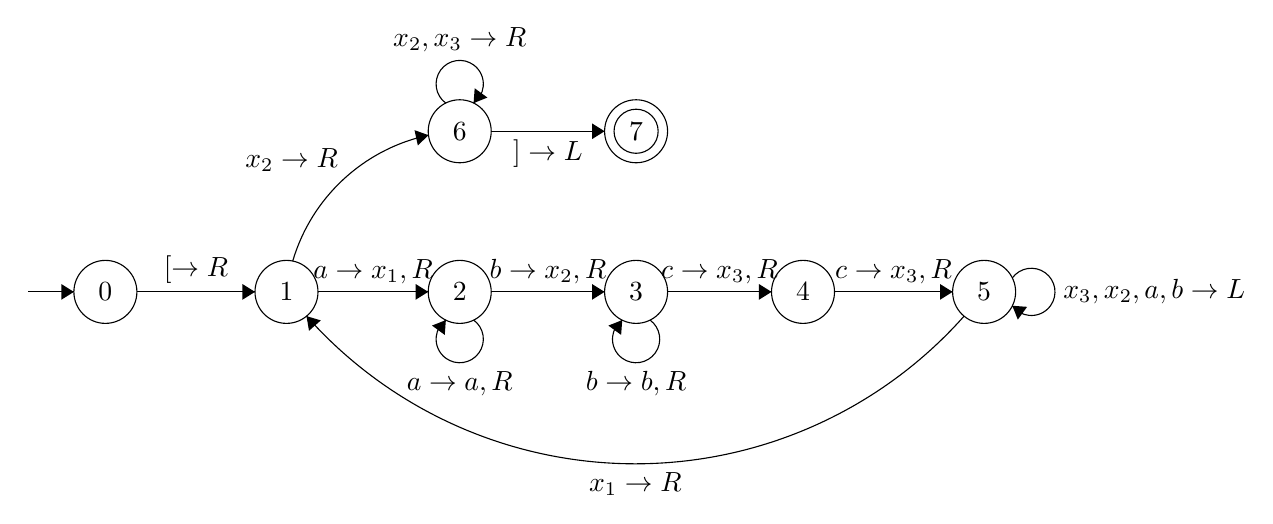
\begin{tikzpicture}[scale=0.2]
    \tikzstyle{every node}+=[inner sep=0pt]
    \draw [black] (5.1,-17.1) circle (2);
    \draw (5.1,-17.1) node {$0$};
    \draw [black] (16.6,-17.1) circle (2);
    \draw (16.6,-17.1) node {$1$};
    \draw [black] (27.6,-17.1) circle (2);
    \draw (27.6,-17.1) node {$2$};
    \draw [black] (38.8,-17.1) circle (2);
    \draw (38.8,-17.1) node {$3$};
    \draw [black] (49.4,-17.1) circle (2);
    \draw (49.4,-17.1) node {$4$};
    \draw [black] (60.9,-17.1) circle (2);
    \draw (60.9,-17.1) node {$5$};
    \draw [black] (27.6,-6.9) circle (2);
    \draw (27.6,-6.9) node {$6$};
    \draw [black] (38.8,-6.9) circle (2);
    \draw (38.8,-6.9) node {$7$};
    \draw [black] (38.8,-6.9) circle (1.4);
    \draw [black] (0.2,-17.1) -- (3.1,-17.1);
    \fill [black] (3.1,-17.1) -- (2.3,-16.6) -- (2.3,-17.6);
    \draw [black] (7.1,-17.1) -- (14.6,-17.1);
    \fill [black] (14.6,-17.1) -- (13.8,-16.6) -- (13.8,-17.6);
    \draw (10.85,-16.6) node [above] {$[\to R$};
    \draw [black] (18.6,-17.1) -- (25.6,-17.1);
    \fill [black] (25.6,-17.1) -- (24.8,-16.6) -- (24.8,-17.6);
    \draw (22.1,-16.6) node [above] {$a\to x_1,R$};
    \draw [black] (28.482,-18.886) arc (54:-234:1.5);
    \draw (27.6,-22.1) node [below] {$a\to a,R$};
    \fill [black] (26.72,-18.89) -- (25.84,-19.24) -- (26.65,-19.83);
    \draw [black] (29.6,-17.1) -- (36.8,-17.1);
    \fill [black] (36.8,-17.1) -- (36,-16.6) -- (36,-17.6);
    \draw (33.2,-16.6) node [above] {$b\to x_2,R$};
    \draw [black] (39.682,-18.886) arc (54:-234:1.5);
    \draw (38.8,-22.1) node [below] {$b\to b,R$};
    \fill [black] (37.92,-18.89) -- (37.04,-19.24) -- (37.85,-19.83);
    \draw [black] (40.8,-17.1) -- (47.4,-17.1);
    \fill [black] (47.4,-17.1) -- (46.6,-16.6) -- (46.6,-17.6);
    \draw (44.1,-16.6) node [above] {$c\to x_3,R$};
    \draw [black] (51.4,-17.1) -- (58.9,-17.1);
    \fill [black] (58.9,-17.1) -- (58.1,-16.6) -- (58.1,-17.6);
    \draw (55.15,-16.6) node [above] {$c\to x_3,R$};
    \draw [black] (62.686,-16.218) arc (144:-144:1.5);
    \draw (65.9,-17.1) node [right] {$x_3,x_2,a,b\to L$};
    \fill [black] (62.69,-17.98) -- (63.04,-18.86) -- (63.63,-18.05);
    \draw [black] (59.626,-18.641) arc (-41.62781:-138.37219:27.929);
    \fill [black] (17.87,-18.64) -- (18.03,-19.57) -- (18.78,-18.91);
    \draw (38.75,-28.52) node [below] {$x_1\to R$};
    \draw [black] (16.997,-15.142) arc (163.56607:102.11177:11.505);
    \fill [black] (25.62,-7.15) -- (24.73,-6.83) -- (24.94,-7.8);
    \draw (16.92,-9.48) node [above] {$x_2\to R$};
    \draw [black] (26.718,-5.114) arc (234:-54:1.5);
    \draw (27.6,-1.9) node [above] {$x_2,x_3\to R$};
    \fill [black] (28.48,-5.11) -- (29.36,-4.76) -- (28.55,-4.17);
    \draw [black] (29.6,-6.9) -- (36.8,-6.9);
    \fill [black] (36.8,-6.9) -- (36,-6.4) -- (36,-7.4);
    \draw (33.2,-7.4) node [below] {$]\to L$};
    \end{tikzpicture}
\caption{Linear Bounded Automaton for \(L=\left\{a^nb^nc^{2n}\mid n\ge 1\right\}\)}
\end{figure}

\subsection{}
We will prove that context-sensitive languages are closed under union, intersection, and concatenation.
Suppose \(M_1\) and \(M_2\) are linear bounded machines recognizing context-sensitive languages \(L_1\) and \(L_2\).
(Throughout this proof, we suppose the alphabet of \(L_1\) and \(L_2\) are the same.)
\begin{align*}
M_1 &= (Q_1, \Sigma, \Gamma_1, q_{0, 1}, q_{acc, 1}, q_{rej, 1})\\
M_2 &= (Q_2, \Sigma, \Gamma_2, q_{0, 2}, q_{acc, 2}, q_{rej, 2})
\end{align*}
\begin{itemize}
\item Union:
We construct the linear-bounded automaton \(M\) for recognizing \(L_1 \cup L_2\).
% \begin{align*}
% M &= (Q, \Sigma, \Gamma, q_{0}, q_{acc}, q_{rej})\\
% \text{Where } Q &= Q_1\times Q_2 \cup \left\{q_0, q_{rej}, q_{acc}, r_1, r_2\right\}\\
% \Gamma_3 &= \Sigma  \cup \Gamma_1 \times \Gamma_2
% \end{align*}
We need to run both machines \(M_1\) and \(M_2\) on the tape and if any of them accepts the string, we accept it.
We design states of \(M\) as Cartesian product of \(Q_1\) and \(Q_2\) (and some extra states that we will need).
At first, the input string is written on the tape.
We iterate through the tape and change every character \(a\) in the tape to \((a, a)\) and come back to the beginning of the tape:
\begin{figure}[H]
\centering
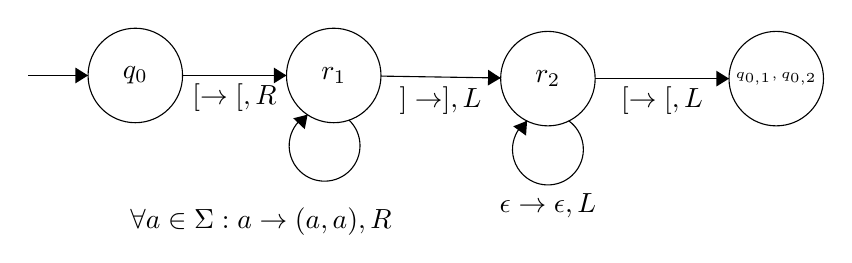
\begin{tikzpicture}[scale=0.2]
    \tikzstyle{every node}+=[inner sep=0pt]
    \draw [black] (7,-3.2) circle (3);
    \draw (7,-3.2) node {$q_0$};
    \draw [black] (19.6,-3.2) circle (3);
    \draw (19.6,-3.2) node {$r_1$};
    \draw [black] (33.2,-3.4) circle (3);
    \draw (33.2,-3.4) node {$r_2$};
    \draw [black] (47.7,-3.4) circle (3);
    \draw (47.7,-3.4) node {{\tiny $q_{0,1}, q_{0, 2}$}};
    \draw [black] (0.2,-3.2) -- (4,-3.2);
    \fill [black] (4,-3.2) -- (3.2,-2.7) -- (3.2,-3.7);
    \draw [black] (10,-3.2) -- (16.6,-3.2);
    \fill [black] (16.6,-3.2) -- (15.8,-2.7) -- (15.8,-3.7);
    \draw (13.3,-3.7) node [below] {$[\to [,R$};
    \draw [black] (20.565,-6.028) arc (46.56859:-241.43141:2.25);
    \draw (14.98,-11.54) node [below] {$\forall a\in \Sigma: a\to (a, a), R$};
    \fill [black] (17.94,-5.69) -- (17.03,-5.92) -- (17.76,-6.61);
    \draw [black] (22.6,-3.24) -- (30.2,-3.36);
    \fill [black] (30.2,-3.36) -- (29.41,-2.84) -- (29.39,-3.84);
    \draw (26.38,-3.85) node [below] {$]\to ], L$};
    \draw [black] (34.523,-6.08) arc (54:-234:2.25);
    \draw (33.2,-10.65) node [below] {$\epsilon\to \epsilon,L$};
    \fill [black] (31.88,-6.08) -- (31,-6.43) -- (31.81,-7.02);
    \draw [black] (36.2,-3.4) -- (44.7,-3.4);
    \fill [black] (44.7,-3.4) -- (43.9,-2.9) -- (43.9,-3.9);
    \draw (40.45,-3.9) node [below] {$[\to [,L$};
    \end{tikzpicture}
\end{figure}
Then we mark both characters of the first pair on the input, denoting the initial positions of two heads.
Then we do the following steps:
\begin{enumerate}
\item Run \(M_1\) on first symbol of the current pair.
Write the symbol on the first symbol of the current pair and move the head in the direction specified by its transition. Mark the first symbol of that pair.
If we are in the state \(q_1, q_2\), after this step we go to the state \(q_1', q_2\) where \(q_1'\) is the state specified by \(M_1\)'s transition.
\item Search for the marked symbol on the second symbol of pairs (e.g., search for it in the left direction and if not found, search for it in the right direction).
\item Run \(M_2\) on the second symbol of the current pair. Move the head, mark the second symbol of that pair and change the (second part of) state similar to step 1.
\item Search for the marked symbol on the first symbol of pairs.
\item Go to step 1.
\item In any step, if we go to any of the states in the set \(\left\{(q_{acc, 1}, r)\mid r \in Q_2\right\} \cup \left\{(r, q_{acc, 2})\mid r \in Q_1\right\}\), we 
go to the state \(q_{acc}\) and accept the string.
\end{enumerate}

So we have constructed an LBA recognizing \(L_1 \cup L_2\) and proved its context-sensitive.

\item Intersection: We do exactly same as the previous part, except the 6\textsuperscript{th} step; we accept the string only if both machines accept it. That means \(q_{acc} = (q_{acc, 1}, q_{acc, 2})\).

\item Concatenation: We construct \(M\) as follows:
\begin{enumerate}
\item Non-deterministically (note that LBAs are non-deterministic), guess the first character of the second part of string (the part that is accepted with \(M_2\)), memorize it and change it to \(]\).
\item Return to the beginning of the tape and run \(M_1\) on the input string.
\item If \(M_1\) rejects, reject. If it accepts the string, we go to the first \(]\) symbol, change it back to the initial character, change the character before it to \([\) and run \(M_2\) on from there.
\item If \(M_2\) rejects, reject. If it accepts the string, we accept it.
\end{enumerate}
So \(L_1 \circ L_2\) is context-sensitive.
\end{itemize}

\section{Recognizability and Decidability}
\subsection{}
It's not decidable.\\
Proof by contradiction:
Suppose it's decidable and \(S\) decides it.
In this case, we design Turing Machine \(U\) deciding the language \(A_{TM}\).\\
\(U = \) ``On input \(\langle M,w \rangle\) where \(M\) is a TM and \(w\) is a string:
\begin{enumerate}[label=\(\arabic*.\)]
\item Construct the following TM, \(M_1\):\\
\(M_1\) = ``On input \(x\):
\begin{enumerate}[label=\(\arabic*.\)]
\item If \(x=1\), accept.
\item If \(x=2\), run \(M\) on \(w\). Accept if \(M\) accepts \(w\).''
\end{enumerate}
\item Construct the following TM, \(M_2\):\\
\(M_2\) = ``On input \(x\):
\begin{enumerate}[label=\(\arabic*.\)]
\item If \(x=1\), accept.
\item If \(x=2\), accept.''
\end{enumerate}
\item Run \(S\) on \(\langle M_1, M_2 \rangle\).
\item If \(S\) accepts, accept. If \(S\) rejects, reject.''
\end{enumerate}

But we know that \(A_{TM}\) is not decidable, so we have a contradiction.

\subsection{}
Suppose \(M_A\) and \(M_B\) are deciders for \(A\) and \(B\), respectively.
\subsubsection{}
We design \(M\), deciding \(A \cup B\), as follows:\\
\(M = \) ``On input \(w\):
\begin{enumerate}
\item Run \(M_A\) on \(w\).
\item If \(M_A\) accepts, accept.
\item If \(M_A\) rejects, run \(M_B\) on \(w\).
\item If \(M_B\) accepts, accept.
\item If \(M_B\) rejects, reject.''
\end{enumerate}

Note that since \(M_A\) and \(M_B\) are deciders, they both halt on any input.

\subsubsection{}
We design \(U\), deciding \(A^*\), as follows:\\
\(U = \) ``On input \(w\):
\begin{enumerate}
\item If \(w = \varepsilon\), accept.
\item For \(n\in \left\{1, 2, \ldots, \abs{w}\right\}\):
    \begin{enumerate}
        \item[] For all possible splits of \(w\) to \(w_1, w_2, \ldots, w_n\):
        \begin{enumerate}
            \item[] Run \(M_A\) on all the strings \(w_1, \ldots, w_n\). If all of them accept, accept.
        \end{enumerate}
    \end{enumerate}
\item If none of the splits accept, reject.''
\end{enumerate}

Since \(U\) has to run \(M_A\) finitely many times, it halts eventually. So it's a decider.

\subsection{}
Suppose \(M_A\) and \(M_B\) are recognizers for \(A\) and \(B\), respectively.

\subsubsection{}
We design \(M\), recognizing \(AB\), as follows:\\
\(M = \) ``On input \(w\):
\begin{enumerate}
\item Non-deterministically guess the first character of the second part of the string.
\item Run \(M_A\) and \(M_B\) on the first and second parts of the string, respectively.
\item If both of them accept, accept.''
\end{enumerate}

\subsubsection{}
We want to prove that \(A\) is Turing Decidable if and only if \(A\) and \(\bar{A}\) are both Turing Recognizable.\\
One of the directions is easy. We know that every decidable language is recognizable too. And complement of a decidable language is decidable. So if \(A\) is decidable, then \(A\) and \(\bar{A}\) are both recognizable.\\
For other direction, suppose \(M_1\) and \(M_2\) are recognizers for \(A\) and \(\bar{A}\), respectively. We design \(M\), deciding \(A\), as follows:\\
\(M = \) ``On input \(w\):
\begin{enumerate}
\item Run both \(M_1\) and \(M_2\) on \(w\) in parallel.
\item If \(M_1\) accepts, accept. If \(M_2\) accepts, reject.''
\end{enumerate}
And running in parallel means having two tapes for simulating \(M_1\) and \(M_2\), taking turn for running one step of each machine.

We know that every string \(w\) is either in \(A\) or \(\bar{A}\). So either \(M_1\) or \(M_2\) accepts \(w\). So \(M\) halts. Therefore, it's a decider.

\subsection{}
\subsubsection{}
Suppose \(A\) is the language \(\left\{w\in \left\{a, b\right\}^*\mid n_a(w) \ge n_b(w)\right\}\).
For the input DFA \(D\), we want to test that \(L(D) \subseteq A\) or equivalently, \(L(D)-A = L(D)\cap \bar{A} = \emptyset\).

We know that \(\bar{A}\) is still a context-free language in this case:
\begin{align*}
\bar{A} = \left\{w\in \left\{a, b\right\}^*\mid n_a(w) < n_b(w)\right\}
\end{align*}
And we can design following PDA for recognizing it:
\begin{figure}[H]
\centering
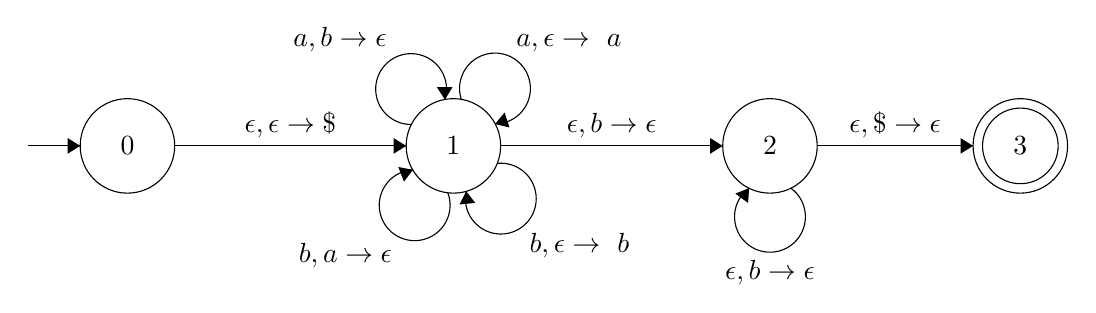
\begin{tikzpicture}[scale=0.2]
    \tikzstyle{every node}+=[inner sep=0pt]
    \draw [black] (6.5,-7.9) circle (3);
    \draw (6.5,-7.9) node {$0$};
    \draw [black] (27.2,-7.9) circle (3);
    \draw (27.2,-7.9) node {$1$};
    \draw [black] (47.3,-7.9) circle (3);
    \draw (47.3,-7.9) node {$2$};
    \draw [black] (63.2,-7.9) circle (3);
    \draw (63.2,-7.9) node {$3$};
    \draw [black] (63.2,-7.9) circle (2.4);
    \draw [black] (0.2,-7.9) -- (3.5,-7.9);
    \fill [black] (3.5,-7.9) -- (2.7,-7.4) -- (2.7,-8.4);
    \draw [black] (9.5,-7.9) -- (24.2,-7.9);
    \fill [black] (24.2,-7.9) -- (23.4,-7.4) -- (23.4,-8.4);
    \draw (16.85,-7.4) node [above] {$\epsilon,\epsilon\to\$$};
    \draw [black] (26.841,-10.867) arc (20.82888:-267.17112:2.25);
    \draw (20.34,-14.05) node [below] {$b,a\to\epsilon$};
    \fill [black] (24.63,-9.42) -- (23.7,-9.24) -- (24.06,-10.17);
    \draw [black] (29.975,-9.01) arc (95.93753:-192.06247:2.25);
    \draw (35.2,-13.41) node [below] {$b,\epsilon\to\mbox{ }b$};
    \fill [black] (28.01,-10.78) -- (27.59,-11.62) -- (28.59,-11.52);
    \draw [black] (24.539,-6.541) arc (270.67261:-17.32739:2.25);
    \draw (20,-1.99) node [above] {$a,b\to\epsilon$};
    \fill [black] (26.66,-4.96) -- (27.15,-4.16) -- (26.15,-4.17);
    \draw [black] (27.701,-4.954) arc (198.08118:-89.91882:2.25);
    \draw (34.53,-1.94) node [above] {$a,\epsilon\to\mbox{ }a$};
    \fill [black] (29.84,-6.51) -- (30.76,-6.73) -- (30.45,-5.78);
    \draw [black] (30.2,-7.9) -- (44.3,-7.9);
    \fill [black] (44.3,-7.9) -- (43.5,-7.4) -- (43.5,-8.4);
    \draw (37.25,-7.4) node [above] {$\epsilon,b\to\epsilon$};
    \draw [black] (48.623,-10.58) arc (54:-234:2.25);
    \draw (47.3,-15.15) node [below] {$\epsilon,b\to\epsilon$};
    \fill [black] (45.98,-10.58) -- (45.1,-10.93) -- (45.91,-11.52);
    \draw [black] (50.3,-7.9) -- (60.2,-7.9);
    \fill [black] (60.2,-7.9) -- (59.4,-7.4) -- (59.4,-8.4);
    \draw (55.25,-7.4) node [above] {$\epsilon,\$\to\epsilon$};
    \end{tikzpicture}
\caption{PDA for recognizing \(\bar{A}\).}
\label{fig:3-4-1}
\end{figure}
And we know that intersection of a context-free language and a regular language is a context-free language.
Suppose \(G\) is our PDA for recognizing \(\bar{A}\).
We design PDA \(G'\), recognizing \(L(D)\cap \bar{A}\), as follows:
\begin{equation}
\begin{aligned}
G &= \left(Q_1, \Sigma, \Gamma, \delta_1, q_1, F_1\right)\\
D &= \left(Q_2, \Sigma, \delta_2, q_2, F_2\right)\\
\implies G' &= \left(Q_1 \times Q_2, \Sigma, \Gamma, \delta', (q_1, q_2), F_1 \times F_2\right)\\
\text{where } \delta'((r_1, r_2), a, b) &= \left\{((q, \delta_2(r_2, a)), s) \mid (q, s) \in \delta_1(r_1, a, b)\right\}
\end{aligned}
\label{eq:3-4-1}
\end{equation}
And finally we know there is a decidable Turing Machine that checks whether language of a CFG is empty or not (denoted by \(E_{CFG}\) in the book).
We use all these to design a decider for \(L\) as follows:\\[7pt]
\(M = \) ``On input \(\left\langle D\right\rangle\):
\begin{enumerate}
\item Construct PDA \(G\) for recognizing \(\bar{A}\) as in Figure \ref{fig:3-4-1}.
\item Construct PDA \(G'\) for recognizing \(L(D)\cap \bar{A}\) as in Equation \eqref{eq:3-4-1}.
\item Convert PDA \(G'\) to an equivalent CFG \(C\) using the algorithm in Section 2.2 of the book.
\item Run \(E_{CFG}\) on \(C\). If it accepts, accept. If it rejects, reject.''
\end{enumerate}

So we have constructed a decider for \(L\).

\subsubsection{}
(\(ALL_{CFG}\) was another language defined in the book!)\\
We use a similar algorithm for deciding this language:
\begin{align*}
L_2 = \left\{\langle D, C\rangle \mid D \text{ is a DFA and } C \text{ is a CFG such that } L(C) \subseteq L(D)\right\}
\end{align*}
We need to make sure \(L(C) \cap \overline{L(D)} = \emptyset\).\\[7pt]
\(M = \) ``On input \(\left\langle D, C\right\rangle\):
\begin{enumerate}
\item Convert DFA \(D\) to DFA \(D'\) which accepts \(overline{L(D)}\), by swapping the final states and the non-final states.
\item Convert CFG \(C\) to the equivalent PDA \(G\), by the algorithm in Section 2.2 of the book.
\item Construct PDA \(G'\) for recognizing \(L(D')\cap L(G)\), as in Equation \eqref{eq:3-4-1}.
\item Convert PDA \(G'\) to an equivalent CFG \(C'\) using the algorithm in Section 2.2 of the book.
\item Run \(E_{CFG}\) on \(C'\). If it accepts, accept. If it rejects, reject.''
\end{enumerate}

So we have constructed a decider for \(L_2\).

\section{Reducibility and Proving Undecidability}

\subsection{}
\subsubsection{}
We want to show that \(Inf_{TM} = \left\{\langle M\rangle\mid L(M) \text{ is infinite}\right\}\) is undecidable.\\
We construct the following machine \(F\) that computes a reduction \(f\) between \(A_{TM}\) and \(Inf_{TM}\):\\[7pt]
\(F = \) ``On input \(\left\langle M, w\right\rangle\):
\begin{enumerate}
\item Construct the following machine \(M'\) as follows:\\
\(M' = \) ``On input \(x\):
\begin{enumerate}[label=\(\arabic*.\)]
\item Run \(M\) on \(w\).
\item If \(M\) accepts, accept. If \(M\) rejects, reject.''
\end{enumerate}
\item  Output \(\left\langle M'\right\rangle\).''
\end{enumerate}

So \(\langle M, w\rangle \in A_{TM} \text{ iff } f(\langle M, w\rangle) = \langle M'\rangle \in Inf_{TM}\).\\
Thus, we have the reduction \(A_{TM} \leq_{m} Inf_{TM}\) and \(Inf_{TM}\) is undecidable.

\subsubsection{}
\href{http://kilby.stanford.edu/~rvg/154/handouts/ambi.html}{Reference} of the proof.\\
We want to prove that \(INTRSCT_{CFG} = \left\{\langle G_1, G_2\rangle\mid G_1 \text{ and } G_2 \text{ are CFGs such that } L(G_1) \cap L(G_2) = \emptyset\right\}\) is undecidable.\\
We prove it using the undecidability of post correspondence problem (PCP).
Suppose we have a set of dominos \(d_1, d_2, \dots, d_n\), where \(d_i=\left[\frac{w_i}{x_i}\right]\) for \(i\in {1, \ldots, n}\).
Construct two Grammars (\(W, X\)) as below:
\begin{align*}
W &\to w_1Wd_1 \mid w_2Wd_2 \mid \cdots \mid w_nWd_n \mid w_1d_1 \mid w_2d_2 \mid \cdots \mid w_nd_n\\
X &\to x_1Xd_1 \mid x_2Xd_2 \mid \cdots \mid x_nXd_n \mid x_1d_1 \mid x_2d_2 \mid \cdots \mid x_nd_n
\end{align*}
We know our dominos have a match, if and only if there is a string that can be generated by both \(W\) and \(X\)
(they will have the same dominos on the right-hand side of the string. And the upper and lower parts of dominos form the same strings).\\
So given a pcp instance, we can map it to a problem of \(\overline{INTRSCT_{CFG}}\) as follows:\\[7pt]
\(F = \) ``On input \(\left\langle d_1, d_2, \dots, d_n\right\rangle\):
\begin{enumerate}
\item Construct CFGs \(X\) and \(W\) as above.
\item Output \(\left\langle X, W\right\rangle\).''
\end{enumerate}

We know that \(\left\langle d_1, d_2, \dots, d_n\right\rangle \in PCP\) iff \(\left\langle X, W\right\rangle \in \overline{INTRSCT_{CFG}}\).\\
So \(PCP\leq_m \overline{INTRSCT_{CFG}}\) and we know that \(PCP\) is undecidable. So \(\overline{INTRSCT_{CFG}}\) and as a result \(INTRSCT_{CFG}\) are undecidable.

\subsubsection{}
\begin{align*}
PAL_{CFG} = \left\{\langle G\rangle \mid G \text{ is a CFG and } L(G) \text{ contains a pallindrome}\right\}.
\end{align*}
Again, we use the undecidability of PCP to prove this part.\\
Suppose an instance of PCP, contains dominos \(d_1, d_2, \dots, d_n\), where \(d_i=\left[\frac{w_i}{x_i}\right]\).
We design the mapping function as follows:\\[7pt]
\(F = \) ``On input \(\left\langle d_1, d_2, \dots, d_n\right\rangle\):
\begin{enumerate}
\item Construct CFG \(G\) with start variable \(S\) and rules as below:
\begin{align*}
S &\to D_1 \mid D_2 \mid \cdots \mid D_n\\
\forall i \in {1, \ldots, n}: D_i &\to w_i S x_i^R \mid w_i x_i^R & (R \text{ means reverse})
\end{align*}
\item Output \(\left\langle G\right\rangle\).''
\end{enumerate}

We know that the input instance has a match if and only if there is a palindrome string in \(L(G)\).
So \(\left\langle d_1, d_2, \dots, d_n\right\rangle \in PCP\) iff \(\left\langle G\right\rangle \in PAL_{CFG}\), hence \(PCP\leq_m PAL_{CFG}\).
And we know \(PCP\) is undecidable. So \(PAL_{CFG}\) is undecidable.

\subsection{}
Proof by contradiction.
Assume \(T\) is decidable.
Let \(M_T\) be a Turing machine that decides it.
We can construct the following decider for \(A_{TM}\):\\[7pt]
\(F = \) ``On input \(\left\langle M, w\right\rangle\):
\begin{enumerate}
\item construct machine \(M'\) as follows:\\
\(M' = \) ``On input \(x\):
\begin{enumerate}[label=\(\arabic*.\)]
\item If \(x = 12\), accept.
\item If \(x = 21\), Run \(M\) on \(w\) and if it accepts, accept. If it rejects, reject.
\end{enumerate}
\item Run \(M_T\) on the input \(\left\langle M', 12\right\rangle\).
\item If \(M_T\) accepts, accept. If \(M_T\) rejects, reject.''
\end{enumerate}
So we have designed a decider for \(A_{TM}\). But we know \(A_{TM}\) is undecidable.
So we have reached a contradiction and \(T\) is undecidable.

\subsection{}
\subsubsection{}
\href{https://www.dcc.fc.up.pt/~acm/ricep.pdf}{Reference} of the proof.\\
Proof by contradiction: Assume \(P\) is a non-trivial property and \(A_P = \left\{\langle M\rangle \mid M \text{has the property } P\right\}\) is decidable and \(H\) is a decider for it.
\begin{align*}
H(x) = \begin{cases}
\text{accept} & \text{if the machine } x \text{ has the property } P\\
\text{reject} & \text{if the machine } x \text{ does not have the property } P
\end{cases}
\end{align*}
Since \(P\) is non-trivial, there is a machine \(Y\) that has the property \(P\) and a machine \(N\) that does not have it.\\
Define machine \(A\) as below:\\[7pt]
\(A = \) on input \(x\):
\begin{enumerate}
\item If \(H\) accepts \(A\), return \(N(x)\).
\item If \(H\) rejects \(A\), return \(Y(x)\).
\end{enumerate}
Now, if \(A\) has the property \(P\), then \(H(A) =\) accept and \(A(x) \equiv N(x)\).
And if \(A\) does not have the property \(P\), then \(H(A) =\) reject and \(A(x) \equiv Y(x)\).
Which is a contradiction in both cases. So \(A_P\) is undecidable.
\subsubsection{}
First, we show that being finite is a non-trivial property for languages.\\
\begin{multicols}{2}
\(Y = \) ``On input \(x\):
\begin{enumerate}
\item Reject.
\end{enumerate}
\(N = \) ``On input \(x\):
\begin{enumerate}
\item Accept.
\end{enumerate}
\end{multicols}
Clearly the language of \(Y\) is finite and the language of \(N\) is infinite.
Thus, being a non-trivial property, we can conclude that \(FINITE = \left\{\langle T\rangle \mid L(T) \text{ is finite}\right\}\) is undecidable.

\end{document}